\chapter{Data Preparation}

\section{Select Data}

\subsection{Rationale for inclusion/exclusion}
% List the data to be included/excluded and the reasons for these decisions

We have utilized a Python code that includes a function for data preparation by calculating the entropy of a set of labels. The entropy function is essential for various learning tasks and provides valuable insights for feature selection, model training, and decision-making processes.
The entropy calculation is performed using the formula in figure 3.1, where:
\begin{itemize}
    \item \textbf{Labels} refer to the set of labels;
    \item \textbf{n} is the number of distinct labels;
    \item \textbf{pi} represents the probability of each label \textbf{i} within the set.
\end{itemize}
To calculate the entropy, figure 3.2, the function first converts the labels to integer indices, ensuring compatibility with subsequent calculations. It then computes the probabilities of each label by counting their occurrences and dividing by the total number of labels. Finally, the entropy is calculated using the probabilities and the logarithmic function.
This data preparation step is valuable for understanding the diversity and distribution of labels within the dataset. By assessing the entropy, informed decisions can be made regarding data preprocessing, feature selection, and modeling strategies. An entropy value of 0 indicates perfect purity, where all labels in the set are the same. Conversely, higher entropy values indicate a more diverse distribution of labels and higher uncertainty in predicting the class or category of an instance.

\begin{figure}%[!h]
\begin{center}
    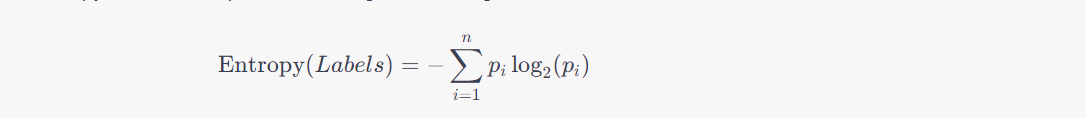
\includegraphics[scale=0.45]{imgs/entropy.png}
    \centering
    \caption{Entropy formula}
    \vspace{15pt}
    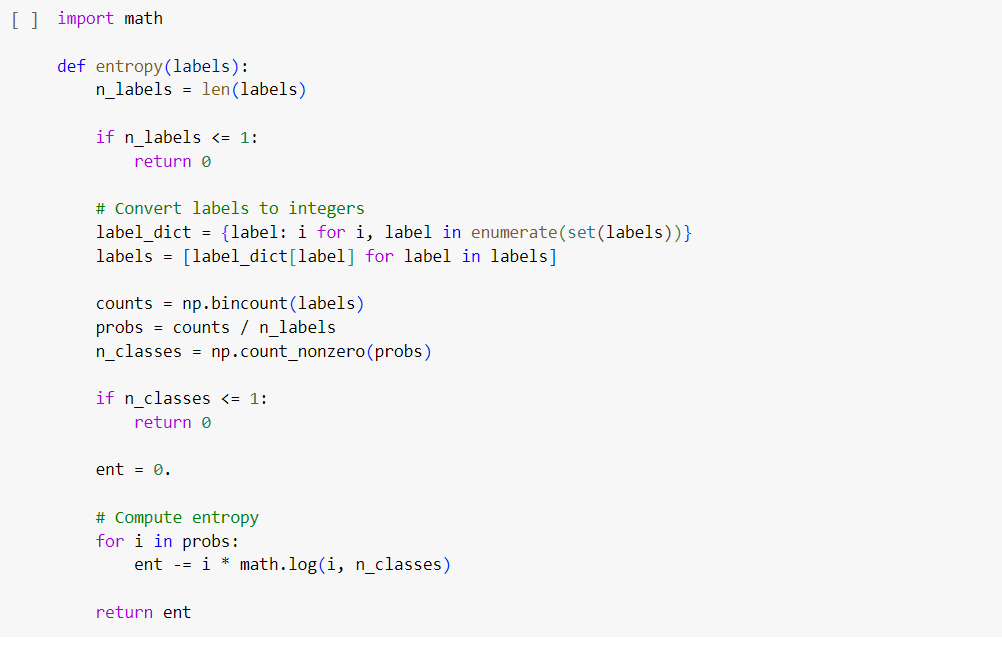
\includegraphics[scale=0.45]{imgs/entropy_function.png}
    \centering
    \caption{Entropy function}
\end{center}
\hrulefill\vspace{15pt}\par
\end{figure}

Based on the above exploratory analysis, a feature subset selection process was conducted to remove features that exhibited low entropy values, figure 3.3. The entropy threshold of 0.2 was set to identify features with limited information gain or relevance to the dataset.
The process involved iterating over each column in the 'housePrice' DataFrame and calculating the entropy for each column using the previously defined entropy() function. If the entropy of a column was found to be below the threshold, it was considered an indicator of low information gain or redundancy.
The selected features, identified through their low entropy values, were printed out, and the 'drop()' method was utilized to remove them from the 'housePrice' DataFrame. This was done by specifying the column name and using the axis=1 parameter to drop the features along the columns.
By removing irrelevant or redundant features, the dimensionality of the dataset was reduced, which can enhance the efficiency and performance of subsequent machine learning algorithms. The aim of this feature selection process was to retain only the most informative features that contribute significantly to the predictive power of the dataset.
This reduction offers advantages such as improved computational efficiency, reduced risk of overfitting, and enhanced interpretability of models. By focusing on the most important predictors, the selected subset may lead to more accurate predictions and better generalization to unseen data.
After performing the feature subset selection, the original data frame, which initially consisted of 81 columns, was reduced to 64 columns, retaining the most informative features.

\begin{figure}[t]
    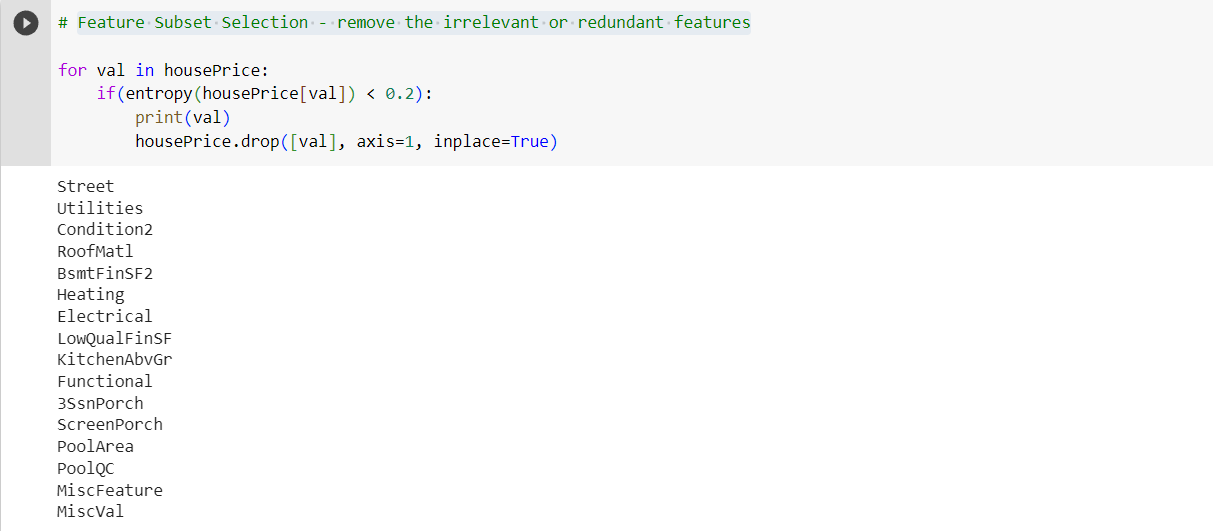
\includegraphics[scale=0.45]{imgs/feature_subset_selection.png}
    \centering
    \caption{Feature subset selection}
    \hrulefill\vspace{15pt}\par
\end{figure}

\section{Clean Data}

Since we have data understanding, we will now do data cleaning.  Data cleaning step is a very crucial step for reliable and better performance of our model in machine learning. In our data cleaning we have identified and removed noises in order to ensure that we have the accurate dataset for analysis. Checked for duplication and missing value on the given dataset of each attribute. 

\subsection{Data Cleaning Report}
% Describe what decisions and actions you took to address data quality problems

\begin{figure}[t]
    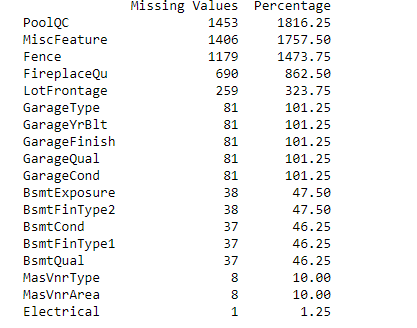
\includegraphics[scale=0.55]{imgs/missing_value.png}
    \centering
    \caption{Missing value}
    \hrulefill\vspace{15pt}\par
\end{figure}

We have 1460 unique Id in our dataset. We have used this Id in order to identify in case of duplicated instances in our dataset. Our dataset is consisting of 1460 rows and 81 columns. Each row Id were unique hence we were able to not use Id for our training set.

Given that for the attribute Alley with value of NA were considered as a value of object and not a missing value, figure 3.4, for the rest of the dataset we have found 18 columns that have missing value, in which the sum value of missing value or null was above 0. In the fig below we can see the attributes in which their missing value was not 0, PoolQC, MiscFeature and Fence having to large amount of missing value.
To remove the missing value, we have replaced the null value with mean value taking example LotFrontafe, GarafeYrBlt and MasVnrArea columns.

We have checked that there is:
\begin{itemize}
    \item Negative value: in our data set we do not have negative values.;
    \item No negative value and now we check if there is duplication, but we have non-unique value on our dataset except the attribute of Id;
    \item Out-of-range values: the attributes we didn’t consider while training out mode are Id and SalePrice. SalePrice was determined by the added PriceLabel, and we did not use it for our training data only when labelling the value on PriceLabel.;
    \item Inconsistency: we didn’t have data inconsistencies;
    \item Duplicate: We have checked that there is no negative value and now we check if there is duplication, but we have non-unique value on our dataset except the attribute of Id. Hence, we have not found any duplication.
\end{itemize}
     

\section{Construct Data}

\subsection{Derived attributes}
% New attriutes constructed from one or more existing attributes

To gain insights into trends and patterns based on the construction year, the 'housePrice' DataFrame is grouped using the 'YearBuilt' column. This grouping creates separate subsets of data for each unique year. The mean() method is then applied to calculate the average values for each numerical attribute within each group. This provides a new DataFrame displaying the average attribute values grouped by the construction year.
By calculating the mean values for each attribute, we can analyze the central tendency or average level of different attributes for each year. This allows us to identify potential relationships or dependencies between the construction year and other quantitative attributes in the dataset.
This information can aid in making informed decisions, such as identifying important features for predictive modeling or understanding the impact of time on attribute values.

\begin{figure}[t]
    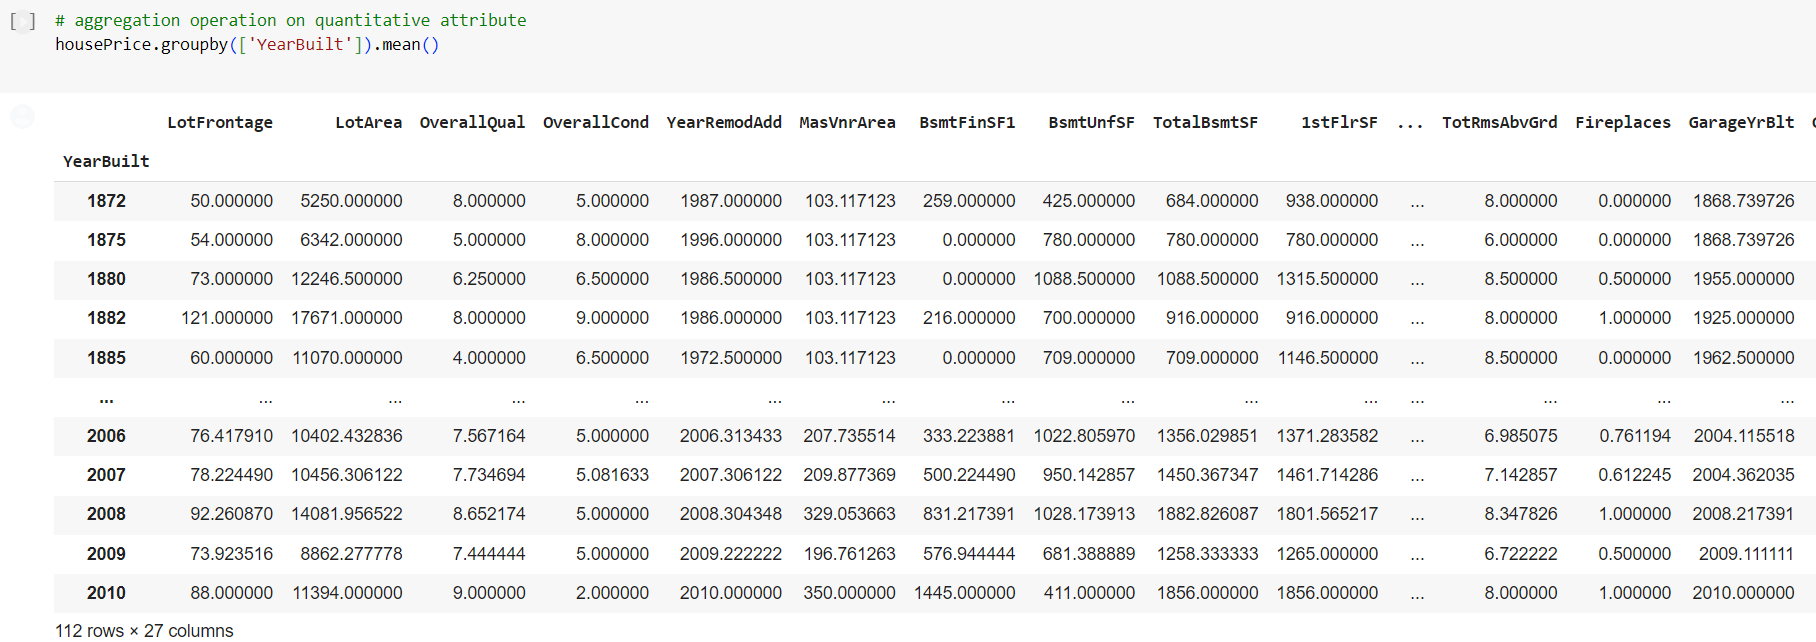
\includegraphics[scale=0.35]{imgs/aggregate_operation.png}
    \centering
    \caption{Aggregate operation}
    \hrulefill\vspace{15pt}\par
\end{figure}


\subsection{Generated records}
% Describe the creation of any completely new records

To capture important information more efficiently in the dataset, a feature creation process was employed by combining the 'OverallQual' and 'OverallCond' attributes. The goal was to generate a new attribute that captures a consolidated measure of the overall quality and condition of the houses. By combining the 'OverallQual' and 'OverallCond' attributes using the addition operator, a new attribute called 'OverallQualCond' was created. This composite feature aims to provide a more comprehensive assessment of each house's overall state, considering both material and finish quality and overall condition.
Following the creation of the 'OverallQualCond' feature, the original 'OverallQual' and 'OverallCond' attributes were dropped from the 'housePrice' DataFrame. This step was taken to remove redundancy and potential multicollinearity issues that could arise from using highly correlated attributes in subsequent modeling tasks, figure 3.5.
As a result of this feature creation process, the modified 'housePrice' DataFrame now includes the newly created 'OverallQualCond' feature while no longer containing the original 'OverallQual' and 'OverallCond' attributes. The inclusion of the 'OverallQualCond' feature provides a consolidated representation of each house's overall quality and condition, potentially offering a more informative and concise feature for analysis and modeling purposes.

\section{Integrate Data}

\subsection{Merged Data}
% To join toghetere two or more tables that have different information about the same objects

In this stage of the data preparation process, there was no need to merge data from multiple sources. The project solely relies on a single dataset, and therefore, there was no requirement to combine or integrate data from different sources.

\begin{figure}%[!h]
\begin{center}
    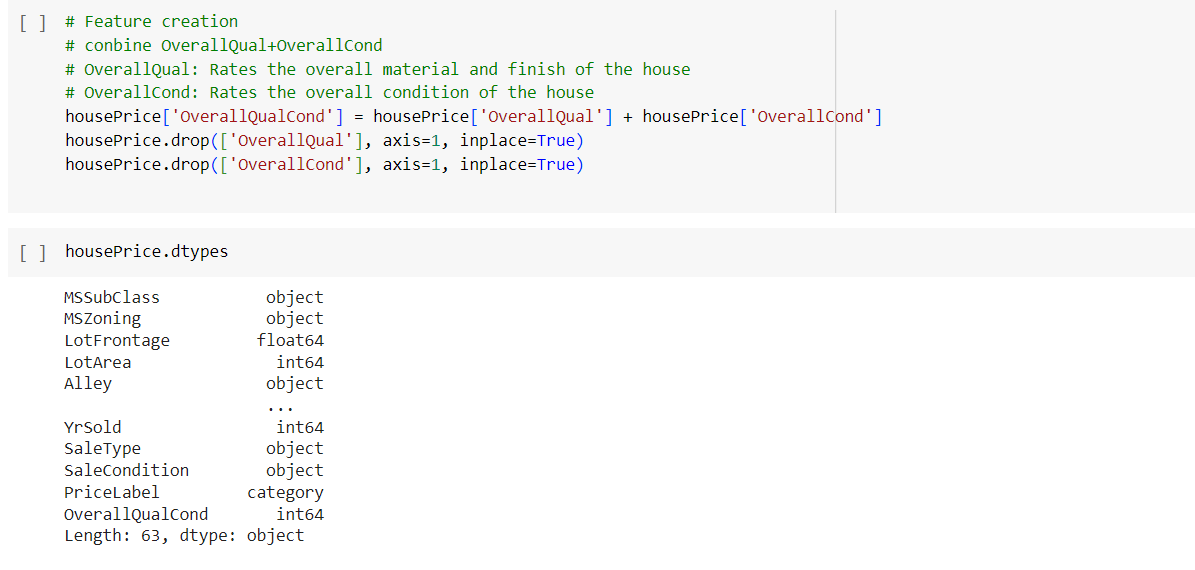
\includegraphics[scale=0.5]{imgs/feature_creation.png}
    \centering
    \caption{Feature creation}
    \vspace{15pt}
    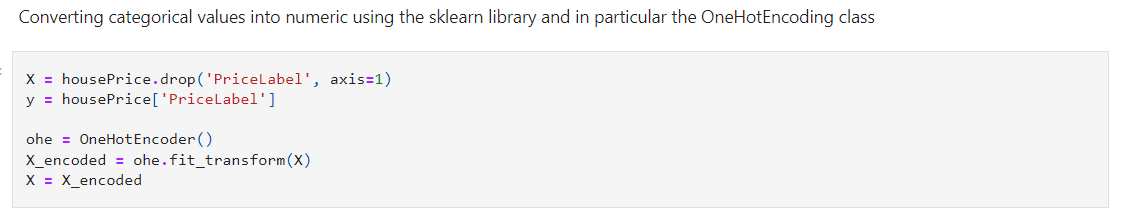
\includegraphics[scale=0.5]{imgs/one_hot_encoder.png}
    \centering
    \caption{OneHotEncoder}
\end{center}
\hrulefill\vspace{15pt}\par
\end{figure}


\section{Format Data}

\subsection{Reformatted Data}
% To satisfy the modeling tool requirementes

In this stage, we have used OneHotEncoder class in scikit-learn for converting our categorical variables into a binary vector representation, figure 3.7, where each category is represented by a separate binary column. This allows the algorithms we have used to consider the presence or absence of each category as a separate feature.
Moreover, the resulting encoded features allow the models to handle categorical data and incorporate it into the learning process, improving the model's ability to capture patterns and make accurate predictions.